\section{Free selective functors}\label{sec-free}

The idea of describing effectful computations using \emph{free constructions},
such as \emph{free}~\cite{swierstra2008data} and \emph{freer
monads}~\cite{kiselyov2015freer} and \emph{free applicative
functors}~\cite{free-applicatives} is well-studied in the functional programming
community. Free constructions allow us to focus on the internal aspects of the
effect under consideration and receive the desired applicative or monadic
computation structure \emph{for free}, i.e. without the need to define custom
instances or prove laws.

In this section we apply this idea to selective functors and present a free
construction for \emph{rigid} selective functors
(\S\ref{sec-free-construction}), which we then demonstrate on several examples.

\subsection{Free construction}\label{sec-free-construction}

In the free structures methodology, the essence of an effect is captured by a
data type that encodes the ``commands'' which the effect provides, acting as a
deep embedding of the effect's interface. This data type needs only have enough
structure to be a~\hs{Functor}. The purpose of a free construction is then to
build a richer structure on top of this \emph{base} functor, which would have
the desired instances, in our case \hs{Applicative} and \hs{Selective}. In this
section we will denote the base functor by \hs{f}.

As we remarked in~\S\ref{sec-laws}, rigid selective functors have a particularly
simple normal form thanks to the additional law \hs{(<*>)}~\hs{=}~\hs{apS},
which tells us that the apply operator \hs{<*>} is redundant and can be
implemented via the selective interface. This normal form has the following
linear structure:

\vspace{1mm}
\begin{minted}[xleftmargin=10pt]{haskell}
pure x <*? fa <*? fb <*? ... <*? fy
  where
    x  :: Either a (Either b (Either c (... z)))
    fa :: f (a ->   Either b (Either c (... z)))
    fb :: f (b ->             Either c (... z))
    ...
    fy :: f (y ->                           z)
\end{minted}
\vspace{1mm}

\noindent
In words, any rigid selective computation can be rewritten as a left-associated
sequence of select operators, where the initial pure value~\hs{x} comes from a
large sum type (comprising alternatives~\hs{a} to~\hs{z} in the above snippet),
and each effect in the sequence of select operators eliminates one of the
alternatives, in order, until only one remains (namely, \hs{z}). Interestingly,
there is no right-associative version of the normal form, because the
associativity law can only be used to re-associate a given expression to the
left. To apply it in reverse, we would need a way to ``factor out'' the
reshaping functions \hs{f}, \hs{g} and \hs{h} from the base functor. This is
different from applicative functors, which have two normal forms corresponding
to left and right re-association~\citep{free-applicatives}.

\begin{figure}
\begin{minted}[fontsize=\small]{haskell}
data Select f a where
    Pure   :: a -> Select f a
    Select :: Select f (Either a b) -> f (a -> b) -> Select f b
\end{minted}
\vspace{1mm}
\begin{minted}[fontsize=\small]{haskell}
instance Functor f => Functor (Select f) where
    fmap f (Pure a)     = Pure (f a)
    fmap f (Select x y) = Select (fmap f <$> x) (fmap f <$> y) -- Free theorem from Fig. 4
\end{minted}
\vspace{1mm}
\begin{minted}[fontsize=\small]{haskell}
instance Functor f => Applicative (Select f) where
    pure  = Pure
    (<*>) = apS -- Law of rigid selective functors
\end{minted}
\vspace{1mm}
\begin{minted}[fontsize=\small]{haskell}
instance Functor f => Selective (Select f) where
    select x (Pure y)     = either y id <$> x -- Generalised identity
    select x (Select y z) = Select (select (f <$> x) (g <$> y)) (h <$> z) -- Associativity
      where
        f x = Right <$> x
        g y = \a -> bimap (,a) ($a) y
        h z = uncurry z
\end{minted}
\vspace{1mm}
\begin{minted}[fontsize=\small]{haskell}
-- Lift a base functor into Select
liftSelect :: Functor f => f a -> Select f a
liftSelect f = Select (Pure (Left ())) (const <$> f)
\end{minted}
\vspace{1mm}
\begin{minted}[fontsize=\small]{haskell}
-- Interpret a free selective structure given a natural transformation from f to g
runSelect :: Selective g => (forall a. f a -> g a) -> Select f a -> g a
runSelect _ (Pure a)     = pure a
runSelect t (Select x y) = select (runSelect t x) (t y)
\end{minted}
\vspace{1mm}
\begin{minted}[fontsize=\small]{haskell}
-- Extract the resulting value from a pure selective computation
getPure :: Select f a -> Maybe a
getPure = runSelect (const Nothing)
\end{minted}
\vspace{1mm}
\begin{minted}[fontsize=\small]{haskell}
-- Extract all possible effects from a selective computation
getEffects :: Functor f => Select f a -> [f ()]
getEffects = getOver . runSelect (Over . pure . void)
\end{minted}
\vspace{-2mm}
\caption{Free rigid selective functors.}\label{fig-free}
\vspace{-3mm}
\end{figure}

Fig.~\ref{fig-free} gives an encoding of this normal form in Haskell. The free
data type \hs{Select} has two constructors: \hs{Pure}, to embed pure values in
a selective computation, and \hs{Select} to build type-aligned sequences of
base functor effects, by appending new effects to the right end of the sequence.
The sequence can only be started with the \hs{Pure} constructor, thus enforcing
the normal form. Implementation of instances relies on the laws presented
in~\S\ref{sec-laws}: generalised identity, associativity, as well as one of the
free theorems. We do not need the distributivity law, since it is subsumed by
the law of rigid selective functors \hs{(<*>)}~\hs{=}~\hs{apS}, which is used
directly in the \hs{Applicative} instance.

Effects from the base functor can be embedded in the free construction using
the helper function \hs{liftSelect}. To interpret a free selective computation
\hs{Select}~\hs{f}~\hs{a} in a selective functor \hs{g}, one needs to provide
a \emph{natural transformation} from \hs{f} to \hs{g} to the function
\hs{runSelect}, which traverses the sequence of effects converting them to
\hs{g} and composing the results using \hs{g}'s select operator.

For example, \hs{getPure} reinterprets a given free computation in the selective
functor \hs{g}~\hs{=}~\hs{Maybe} using the natural transformation
\hs{const}~\hs{Nothing}, which leaves the \hs{Pure} head of the sequence as is,
but turns any subsequent effect into \hs{Nothing}. Similarly, \hs{getEffects}
records all effects by stashing them in the selective functor \hs{Over}, which
are subsequently extracted from it by \hs{getOver}.

We do not present a free construction for non-rigid selective functors, since it
is more complex and not particularly enlightening.
% In the rest of the section
% we demonstrate applications of free rigid selective functors.

\subsection{Ping-pong, freely}\label{sec-free-ping-pong}

To illustrate the usage of the free selective functors on a simple example,
we implement the classic \cmd{Teletype} DSL~\cite{swierstra2008data} comprising
two commands: reading a string form the input stream and writing a string to the
output stream. The base functor has two corresponding constructors:

\vspace{1mm}
\begin{minted}[xleftmargin=10pt]{haskell}
data Teletype a = Get (String -> a) | Put String a deriving Functor
\end{minted}
\vspace{1mm}

\noindent
For convenience, we provide the following functions that embed the commands into
the free selective construction, mimicking Haskell's \hs{IO} API:

\vspace{1mm}
\begin{minted}[xleftmargin=10pt]{haskell}
getLine :: Select Teletype String
getLine = liftSelect (Get id)
\end{minted}
\vspace{1mm}
\begin{minted}[xleftmargin=10pt]{haskell}
putStrLn :: String -> Select Teletype ()
putStrLn s = liftSelect (Put s ())
\end{minted}
\vspace{1mm}

\noindent
We can now reimplement the \hs{pingPongS} example from~\S\ref{sec-intro} in
terms of the free selective construction simply by adjusting the type signature:

\vspace{1mm}
\begin{minted}[xleftmargin=10pt]{haskell}
pingPongS :: Select Teletype ()
pingPongS = whenS (fmap ("ping"==) getLine) (putStrLn "pong")
\end{minted}
\vspace{1mm}

\noindent
By embedding \hs{pingPongS} into the free construction, we gain access to the
static analysis machinery:

\vspace{1mm}
\begin{minted}[xleftmargin=10pt]{haskell}
@\ghci@ getEffects pingPongS
[Get,Put "pong"]
\end{minted}
\vspace{1mm}

\noindent
The \hs{getEffects} function (Fig.~\ref{fig-free}) returns a list of all effects
of a free selective computation. In the case of the \hs{Teletype} functor, we
get a list of all commands that a computation might execute.

% Internally, the \hs{getEffects} function interprets a free selective computation
% in the \hs{Over} functor (see section~\ref{sec-instances}) to construct an over-approximated
% list of effects.

We can interpret \cmd{Teletype} programs in any other selective functor using
the \hs{runSelect} function by providing a natural transformation
\hs{forall}~\hs{a.}~\hs{Teletype}~\hs{a}~\hs{->}~\hs{g}~\hs{a}, which assigns an
interpretation to \cmd{Teletype} commands in terms of \hs{g}. A good example of
such transformation would be an interpretation in the \hs{IO} monad, which
allows us to execute our \hs{pingPongS} program:

\vspace{1mm}
\begin{minted}[xleftmargin=10pt]{haskell}
toIO :: Teletype a -> IO a
toIO (Get f)   = f <$> Prelude.getLine
toIO (Put s a) = a <$  Prelude.putStrLn s
\end{minted}
\vspace{1mm}
\begin{minted}[xleftmargin=10pt]{haskell}
@\ghci@ runSelect toIO pingPongS
hello
@\ghci@ runSelect toIO pingPongS
ping
pong
\end{minted}
\vspace{1mm}

% Software build systems can be modelled with purely functional
% abstractions~\cite{mokhov2018build} that enable the model to accommodate many
% different build systems and express their features in a way that allow for deriving
% new build systems by combining the best parts of the existing ones. The approach
% presented on~\cite{mokhov2018build} allows to distinguish the \emph{static} build
% dependencies from the \emph{dynamic} ones by expressing the build tasks which
% may only have static dependencies with the \hs{Applicative} interface, and using
% \hs{Monad} for constructing build tasks with dynamic dependencies.
% As selective functors give us the best of both worlds, we show how we could adopt
% their free construction to build a deep embedding of the \hs{fetch} callback from
% the original paper.

% To use any free construction, we need to invent an underlying functor, which would
% be the essence of the effect we are trying to implement. In case of the \hs{fetch}
% callback, we require an effect of a read-only store:

% \begin{minted}[xleftmargin=10pt]{haskell}
% data Fetch k v a = Fetch k (v -> a)
%    deriving Functor
% \end{minted}

% That is, the \hs{Fetch} functor has only one data constructor, which represents a
% command with a suggested semantics of extracting a value associated with a key from
% the store.

% We cannot directly use the \hs{Fetch} command in a selective computations, thus we
% embed it into a free selective construction by simply lifting the data constructor
% in the following way:

% \begin{minted}[xleftmargin=10pt]{haskell}
% fetch :: k -> Select (F k v) v
% fetch key = liftSelect $ Fetch key id
% \end{minted}

\subsection{Analysis and simulation of processor instructions}\label{sec-free-isa}

To demonstrate the free construction on a more interesting example, we apply it
to analysis and simulation of a hypothetical instruction set architecture
(ISA)\footnote{Incidentally, this was the original motivation for selective
functors: while describing the formal semantics of instructions of a real
processor, we needed a statically analysable \hs{ifS} combinator, which
eventually led us to \hs{select}. We use a hypothetical ISA in this section
instead of the real one, because of the complexity of the latter.}. By
expressing the ISA semantics in our free construction, we will be able to build
tools both for static data-flow analysis, and sequential program simulation.

\subsubsection{ISA semantics}

We represent the semantics of instructions using the following data type:

\vspace{1mm}
\begin{minted}[xleftmargin=10pt]{haskell}
type ISA a = Select RW a
\end{minted}
\vspace{1mm}
\begin{minted}[xleftmargin=10pt]{haskell}
data RW a = Read  Key             (Value -> a)
          | Write Key (ISA Value) (Value -> a)
    deriving Functor
\end{minted}
\vspace{1mm}

\noindent

The \hs{RW} (pronounced ``read-write'') functor encodes the effect of a mutable
key-value store comprising two commands: (i) we need the ability to \emph{read}
a value associated with a key from the store, and (ii) given a computation which
produces a value, \emph{write} its result into the store. In this example, we
fix the values to be machine words and the keys to be various ISA memory
locations, such as registers, memory cells and processor status flags.

This exact structure of the definition is required for accommodating a pattern
that occurs frequently in instruction semantics: often we read a value from a
register or a memory cell, do something with it, and then write it somewhere
else. If \hs{Write} required the second argument to be a pure value, as
\cmd{Teletype}'s \hs{Put}, we would not be able to express the desired pattern
without resorting to the monadic interface. Additionally, we want the \hs{Write}
command to not just write the value and return \hs{()}, but to give the just
written value back, so it can be used in the rest of the computation; such
generosity of the \hs{Write} command will be useful for avoiding duplicating
data dependencies.

We introduce two convenience combinators, which lift the data constructors of
the \hs{RW} data type into the free selective, thus making them directly usable
in the definitions of instruction semantics:

\vspace{1mm}
\begin{minted}[xleftmargin=10pt]{haskell}
read :: Key -> ISA Value
read k = liftSelect (Read k id)
\end{minted}
\vspace{1mm}
\begin{minted}[xleftmargin=10pt]{haskell}
write :: Key -> ISA Value -> ISA Value
write k p = p *> liftSelect (Write k p id)
\end{minted}
\vspace{1mm}

\noindent
While the \hs{read} combinator is exactly the lifted \hs{Read} data
constructor, the \hs{write}'s implementation deviates from the trivial lifting
of the \hs{Write} data constructor and \emph{evaluates its second argument},
thus executing the associated effects.

\subsubsection{Example 1. Addition}

To get acquainted with the introduced vocabulary, we start by describing the
semantics for the addition instruction, which reads the summands from a
register and a memory cell, adds them, writes the result back into the register,
and also updates the state of the \hs{Zero} flag to indicate if the result is
zero:

\vspace{1mm}
\begin{minted}[xleftmargin=10pt]{haskell}
add :: Register -> Address -> ISA Value
add reg addr = let arg1     = read (Reg reg)
                   arg2     = read (Mem addr)
                   result   = (+)  <$> arg1   <*> arg2
                   isZero   = (==) <$> pure 0 <*> write (Reg reg) result
               in write (F Zero) (bool 0 1 <$> isZero)
\end{minted}
\vspace{1mm}

\noindent
Here, we \hs{read} the summands \hs{arg1} and \hs{arg2} from the two specified
locations and calculate the \hs{result} of addition by lifting \hs{(+)} into the
free selective functor using applicative combinators. We then calculate the
value of the \hs{Zero} flag in a similar way, but here we exploit the fact that
the \hs{write} combinator returns the value it has just written, thus we can
reuse the \hs{result} without recalculating it from scratch and triggering the
associated effects again.

% The free selective functor construction (\S\ref{sec-free-construction}) shines
% in the static analysis.

By analysing the free semantics of the \hs{add} instruction, we can obtain the
list of all its effects, in the order they appear in the computation. We also
visualise the effects as a data flow graph, where data locations are shown in
rectangles, and instructions in rounded rectangles, with arcs denoting reads
and writes; we denote registers with green \cmd{reg} label, memory addresses
with blue \cmd{address} and flags with the red Unicode flag character.

% \footnote{For didactic purposes,
% these graph was hand-crafted, but it is possible to get similar results automatically
% with Graphviz~\cite{ellson2001graphviz}.}

\vspace{-1mm}
\begin{figure}[!h]
\begin{minipage}{0.45\textwidth}
\raggedleft
\begin{minted}[xleftmargin=10pt]{haskell}
@\ghci@ getEffectsISA (add R0 1)
[Read R0,Read 1,Write R0,Write Zero]
\end{minted}
  % \captionof{listing}{Sub caption}
 \end{minipage}
 \begin{minipage}{0.45\textwidth}
  \centering
  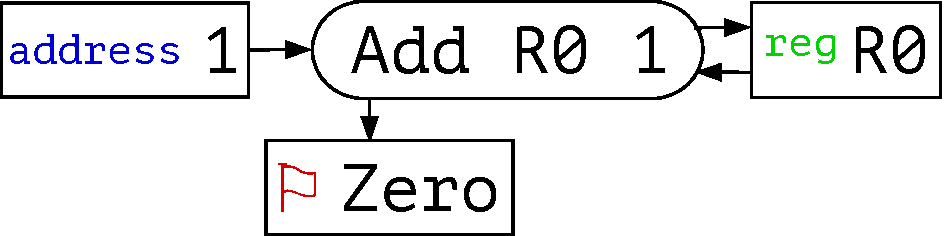
\includegraphics[width=7cm]{./fig/add.pdf}
  % \captionof{listing}{Another sub caption}
 \end{minipage}
 % \captionof{listing}{SomeCaption}
 %  \label{lst:representation_examples}
\end{figure}
\vspace{-1mm}

The semantics of the addition instruction has only used applicative combinators
and we thus could have analysed it statically using free applicative functors.
However, there are important instructions whose semantics cannot be expressed
in terms of the \hs{Applicative} interface, and this is where the presented
free selective construction becomes irreplaceable.

\subsubsection{Example 2. Conditional jump}

Selective functors allow us to introduce limited dependencies between
effectful computations. It turns out that they give just enough power to
express the semantics of conditional jump instructions, which modify the program
counter by a given offset if a certain processor flag is set. As an example,
consider the following instruction that performs a jump if the result of the
previous operation was zero:

\vspace{1mm}
\begin{minted}[xleftmargin=10pt]{haskell}
jumpZero :: Value -> ISA ()
jumpZero offset = let pc       = read PC
                      zeroSet  = (/=) <$> pure 0 <*> read (F Zero)
                      modifyPC = void $ write PC ((+offset) <$> pc)
                  in whenS zeroSet modifyPC
\end{minted}
\vspace{1mm}

\noindent
Here we use the \hs{whenS} combinator to modify the program counter only if
the \hs{Zero} flag is set. By implementing this semantics in terms of the
selective interface, we achieve both the ability to implement an adequate
simulator for the ISA and to retain the possibilities for static analysis of
programs by means of the \hs{getEffectsISA} function:

\begin{figure}[!h]
 \begin{minipage}{0.45\textwidth}
\raggedleft
\begin{minted}[xleftmargin=10pt]{haskell}
@\ghci@ getEffectsISA (jumpZero 42)
[Read Zero,Read PC,Write PC]
\end{minted}
  % \captionof{listing}{Sub caption}
 \end{minipage}
 \begin{minipage}{0.45\textwidth}
  \centering
  
\includegraphics[width=7cm]{./fig/jumpZero.pdf}
  % \captionof{listing}{Another sub caption}
 \end{minipage}
 % \captionof{listing}{SomeCaption}
 %  \label{lst:representation_examples}
\end{figure}

\noindent
Since the analysis is static, the resulting list of effects and the
corresponding data flow graph are over-approximated and show all effects that
can possibly happen in the computation.

% Note that it does not matter which
% argument we supply to \hs{jumpZero}, since it will
% never get forced, e.g. the analysis will succeed and give us the same result even
% if we supply \hs{undefined}.

\subsubsection{Blocks of instructions}

Once we have implemented the semantics for a desired subset of an ISA, we can
describe the semantics of sequences, or \emph{blocks}, of instructions by
simply composing \hs{ISA} computations using the applicative sequencing operator
\hs{*>}:

\vspace{1mm}
\begin{minted}[xleftmargin=10pt]{haskell}
addAndJump :: ISA Value
addAndJump = add R0 1 *> jumpZero 42
\end{minted}
\vspace{1mm}

\noindent
We can analyse the compound computation in the same way we analyse individual
instructions:

\vspace{-3mm}
\begin{figure}[!h]
 \begin{minipage}{0.45\textwidth}
\raggedleft
\begin{minted}[xleftmargin=10pt]{haskell}
@\ghci@ getEffectsISA addAndJump
[Read R0,Read 1,Write R0,Write Zero
,Read Zero,Read PC,Write PC]
\end{minted}
  % \captionof{listing}{Sub caption}
 \end{minipage}
 \begin{minipage}{0.45\textwidth}
  \centering
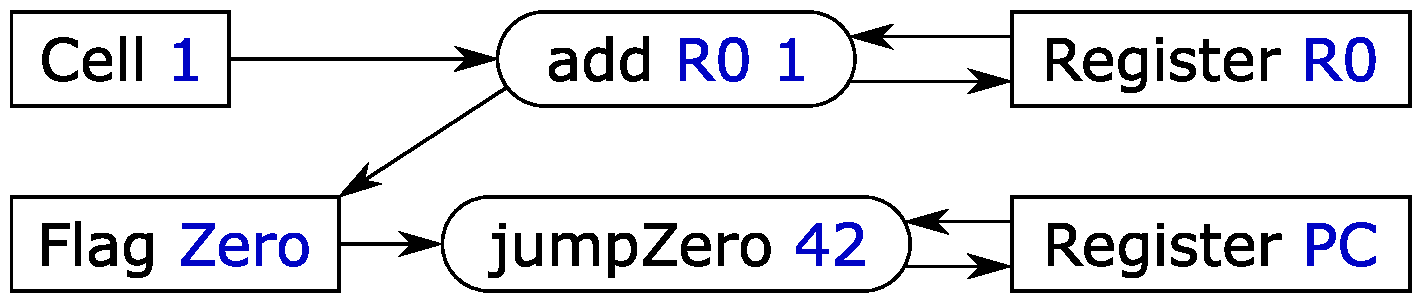
\includegraphics[width=7cm]{./fig/addAndJump.pdf}
  % \captionof{listing}{Another sub caption}
 \end{minipage}
 % \captionof{listing}{SomeCaption}
 %  \label{lst:representation_examples}
\end{figure}

% Getting a flat list of effects that blocks of code perform is not very useful,
% since they does not carry any explicit data-flow information. To mitigate this
% restriction, we take the following approach. We create a (1) deeply-embedded
% assembly language and (2) implement an interpreter which assigns a semantics to
% this language in terms of the free selective construction. By doing this, we can
% then implement a mechanical procedure which would construct \emph{data flow
% graphs} of sequences of instructions, similar to the ones shown in
% Fig.~\ref{fig-addAndJump-gcd} by overlaying the graphs for single instructions.
% Note that if an instruction performs multiple read/writes of the same location,
% we will deliberately merge them in the resulting graph.

\subsubsection{Simulation}

To implement a sequential simulator for the ISA, we need to follow the same path
as in the \hs{pingPongS} example and the \hs{IO} monad earlier in this section.
We need a natural transformation from the functor \hs{RW} to an appropriate
target functor, for example, an instance of \hs{MonadState}~\hs{ISAState},
where \hs{ISAState} is a product type representing the state of the
architecture, e.g. the registers, memory and flags. For brevity, we present a
partial implementation of such a transformation which only assigns an
interpretation to reading and writing registers:

\vspace{1mm}
\begin{minted}[xleftmargin=10pt]{haskell}
toState :: MonadState ISAState m => RW a -> m a
toState (Read k t) = t <$> case k of
    Reg r -> (Map.!) <$> gets registers <*> pure r
    ...
toState (Write k p t) = case k of
    Reg r -> do v <- runSelect toState p
                let regs' s = Map.insert r v (registers s)
                state (\s -> (t v, s {registers = regs' s}))
    ...
\end{minted}
\vspace{1mm}

To read a register, we simply lift the \hs{Data.Map} lookup function (the
register bank is as a mapping from register names to data words). We need to
apply the continuation \hs{t}~\hs{::}~\hs{Value}~\hs{->}~\hs{a} to the result
to make the types match. In order to write an effectful value \hs{p} into a
register, we need to evaluate it first; hence we call the \hs{runSelect}
function, which internally makes a recursive call to the \hs{toState} function
and thus acknowledges the effects of \hs{p}. We then adjust the register bank
with the new value and construct a \hs{MonadState} computation with the
\hs{state} function.

The natural transformation \hs{toState} gives interpretation to individual
\hs{Read} and \hs{Write} commands, and now this interpretation can be extended
to any \hs{ISA} computation by plugging it into a \hs{runSelect} call, as has
already been done once in the implementation of \hs{toState} itself.

\vspace{1mm}
\begin{minted}[xleftmargin=10pt]{haskell}
runProgram :: ISA a -> ISAState -> (a, ISAState)
runProgram f s = runState (runSelect toState f) s
\end{minted}
\vspace{1mm}

\subsubsection{Restrictions}

The free selective construction in combination with the \hs{RW} functor provides
an abstraction capable of expressing the semantics of arithmetical, load and
store instructions, and conditional jumps. However, one should remember that
selective functors still lack the full expressive power of the monadic interface
and are unable to accommodate an important class of instructions, specifically
the instructions that use the memory-indirect addressing mode. If we had a
\hs{Monad} instance for \hs{ISA}, we could have written the following
semantics for the memory-indirect load instruction \hs{loadMI}:

\vspace{1mm}
\begin{minted}[xleftmargin=10pt]{haskell}
loadMI :: Register -> Address -> ISA Value
loadMI reg addr =
    read (Mem addr) >>= \x -> write (Reg reg) (read (Mem (toAddress x)))
\end{minted}
\vspace{1mm}

\noindent
Here, we read from a memory cell, then use the monadic bind operator to extract
a value from the \hs{ISA} type constructor, and use it in a subsequent memory
read. Although this semantics is, in principle, implementable using the
selective \hs{bindS} combinator (see \S\ref{sec-alt-multi}), it is not very
useful in practice since static analysis would record possible access to
\emph{all memory cells}, and there are too many of them (typically, a large
power of two). Furthermore, the execution of the resulting semantics would be
terribly slow, since it would also follow the same linear exploration of the
memory address space. See \S\ref{sec-alt-multi} for a possible solution of this
issue.

% not get any strong benefits. Specifically, since the \hs{getEffectsISA} function, which
% performs static analysis of effects, constructs a conservative over-approximation, it
% would always report something similar to this: \hs{[Read addr,Write reg, Write reg...},
% which would contain as much instances of the \hs{Write} effects as much inhabitants there
% are in the address datatype (usually a large power of two). Therefore, we lose static analysis.
% Maybe we could get some benefit in simulation? No, unfortunately we, again, will not, since
% \hs{bindS} cannot get magically translated to the monadic \hs{>>=}, but instead performs
% explicit enumeration of inhabitants of the bound variable's type, which causes terrible performance regression comparing to a monadic implementation. Considering these arguments,
% using \hs{bindS} for mimicking monadic behaviour is not feasible in our case and memory-indirect
% load cannot be modelled in by means of the \hs{ISA} datatype.
